\documentclass[12pt,aspectratio=169]{beamer}

% ====================================================
% ====================================================
% USEPACKAGES AND IMPORTS
% ====================================================
% ====================================================

\usepackage[T1]{fontenc}
\usepackage[utf8]{inputenc}
\usepackage[english]{babel}

% tables
\usepackage{tabularx}
\usepackage{colortbl}
\usepackage{multirow}
\usepackage{makecell}

% tikz and colors
\usepackage{tikz}
\usepackage{xcolor}
\usepackage{pgfplots}
\usepackage{pgfplotstable}
\usepackage{tikzsymbols}

\usetikzlibrary{calc}
\usetikzlibrary{trees}
\usetikzlibrary{patterns}
\usetikzlibrary{shadings}
\usetikzlibrary{positioning}
\usetikzlibrary{intersections}
\usepgfplotslibrary{patchplots}
\usepgfplotslibrary{fillbetween}
\usetikzlibrary{decorations.pathreplacing}

\usetikzlibrary{arrows}
\usetikzlibrary{arrows.meta}

\usetikzlibrary{shapes}
\usetikzlibrary{shapes.arrows}
\usetikzlibrary{shapes.callouts}
\usetikzlibrary{shapes.symbols}
\usetikzlibrary{shapes.geometric}

% boxes
\usepackage[many]{tcolorbox}

% math packages and fonts
\usepackage{bm}
\usepackage{ccfonts}
\usepackage{eulervm}
\usepackage{amsmath}
\usepackage{amsfonts}
\usepackage{amssymb}
\usepackage{amsthm}
\usepackage{mathtools}
\usepackage{nicefrac}
\usepackage{slashed}
\usepackage{bbold}
\usepackage{array}
\usepackage{cancel}

% algorithms and listings
\usepackage[ruled,vlined,linesnumbered]{algorithm2e}
\usepackage{listings}
\usepackage{setspace}

\tcbuselibrary{listings}
\tcbuselibrary{breakable}
\tcbuselibrary{skins}

% misc
\usepackage{soul}
\usepackage{pifont}
\usepackage{skull}
\usepackage{multicol}
\usepackage{animate}
\usepackage{hyperref}
\usepackage{wasysym}
\usepackage[absolute,overlay]{textpos}
\usepackage[hang,flushmargin]{footmisc}

% ====================================================
% ====================================================
% LAYOUT AND THEME
% ====================================================
% ====================================================

\usetheme{Copenhagen}

% color definitions
\definecolor{myblue1}{RGB}{35,119,189}
\definecolor{myblue2}{RGB}{95,179,238}
\definecolor{myblue3}{RGB}{129,168,207}
\definecolor{myblue4}{RGB}{26,89,142}

\definecolor{myred1}{RGB}{247,12,12}

% set theme colors
\setbeamercolor*{structure}{fg=myblue1,bg=blue}
\setbeamercolor*{palette primary}{use=structure,fg=white,bg=structure.fg}
\setbeamercolor*{palette secondary}{use=structure,fg=white,bg=structure.fg!75!black}
\setbeamercolor*{palette tertiary}{use=structure,fg=white,bg=structure.fg!50!black}
\setbeamercolor*{palette quaternary}{fg=black,bg=white}

\setbeamertemplate{itemize item}[circle]
\setbeamertemplate{itemize subitem}[circle]
\setbeamertemplate{itemize subsubitem}[circle]

\setbeamertemplate{enumerate item}[circle]
\setbeamertemplate{enumerate subitem}[circle]
\setbeamertemplate{enumerate subsubitem}[circle]

\setbeamercolor{itemize item}{fg=myblue1}
\setbeamercolor{itemize subitem}{fg=myblue1}
\setbeamercolor{itemize subsubitem}{fg=myblue1}

\setbeamertemplate{section in toc}[circle]
\setbeamertemplate{subsection in toc}[circle]
\setbeamerfont{subsection in toc}{size=\scriptsize}

\setbeamercolor{frametitle continuation}{fg=black}

% title graphic -- sap logo and dhbw logo
\titlegraphic{
\includegraphics[scale=0.1]{../03_img/logo_sap}\hspace*{4.75cm}~%
   	
\includegraphics[scale=0.05]{../03_img/logo_dhbw}
}

\makeatletter
% frame title
\defbeamertemplate*{frametitle}{mydefault}[1][left]
{
  	\ifbeamercolorempty[bg]{frametitle}{}{\nointerlineskip}%
  	\nointerlineskip%
 	\@tempdima=\textwidth%
  	\advance\@tempdima by\beamer@leftmargin%
  	\advance\@tempdima by\beamer@rightmargin%
  	\begin{tcolorbox}[
  		enhanced,
  		outer arc=0pt,
  		arc=0pt,
  		boxrule=0pt,
  		top=0pt,
  		bottom=0pt,
  		enlarge left by=-\beamer@leftmargin,
  		enlarge right by=-\beamer@rightmargin,
  		width=\paperwidth,
  		nobeforeafter,
  		interior style={
    			left color=myblue2,
    			right color=white
    		},
  		shadow={0mm}{-0.4mm}{0mm}{black!60,opacity=0.6},    
  		shadow={0mm}{-0.8mm}{0mm}{black!40,opacity=0.4},    
  	]
    	\usebeamerfont{frametitle}%
    	\vbox{}\vskip-1ex%
    	\if@tempswa\else\csname beamer@fte#1\endcsname\fi%
    	\insertframetitle\par%
    	{%
      		\ifx\insertframesubtitle\@empty%
      		\else%
      		{\usebeamerfont{framesubtitle}\usebeamercolor[fg]{black}\insertframesubtitle\strut\par}%
      		\fi
    	}%
    	\vskip-1ex%
    	\if@tempswa\else\vskip-.3cm\fi
  	\end{tcolorbox}%
}

% footline of a frame
\defbeamertemplate*{footline}{mysplit theme}
{%
  	\leavevmode%
  	\hbox{
		\begin{beamercolorbox}[
			wd=.5\paperwidth,ht=2.5ex,dp=1.125ex,leftskip=.3cm plus1fill,rightskip=.3cm
		]{author in head/foot}%
    			\usebeamerfont{author in head/foot}\insertshortauthor\ (\insertinstitute), \insertdate
  		\end{beamercolorbox}%
  		\begin{beamercolorbox}[
			wd=.5\paperwidth,ht=2.5ex,dp=1.125ex,leftskip=.3cm,rightskip=.3cm plus1fil
		]{title in head/foot}%
    			\usebeamerfont{title in head/foot}\insertshorttitle\hfill
    			\insertprefix-\insertframenumber/\inserttotalframenumber\hspace*{0.5em}
  		\end{beamercolorbox}}%
  	\vskip0pt%
}
\makeatother

% ====================================================
% ====================================================
% COMMANDS AND GENERAL DEFINITIONS
% ====================================================
% ====================================================

% page number prefix
\newcommand\insertprefix{}  % empty by default
\newcommand\prefix[1]{\renewcommand\insertprefix{#1}}

% math definitions
% ====================================================
\DeclareMathOperator*{\argmax}{arg\,max}
\DeclareMathOperator*{\argmin}{arg\,min}
\newcommand*\diff{\mathop{}\!\mathrm{d}}

\newcommand*{\vertbar}{\rule[-1ex]{0.5pt}{2.5ex}}
\newcommand*{\horzbar}{\rule[.5ex]{2.5ex}{0.5pt}}

% commands
% ====================================================

% highlight commands
% --------------------------------------------------------------------------------------------------------
% highlight command
\newcommand{\highlight}[1]{\textcolor{myblue1}{\textbf{#1}}}
\newcommand{\highlighttt}[1]{\textcolor{myblue1}{\texttt{#1}}}
\newcommand{\Highlight}[1]{\textcolor{myred1}{\textbf{#1}}}

% blue color boxes (with frame/without frame/without fill)
\newtcolorbox{boxBlue}{colback=myblue1!10!white,colframe=myblue4}
\newtcolorbox{boxBlueNoFrame}{colback=myblue1!10!white,colframe=myblue1!10!white}
\newtcolorbox{boxBlueNoFill}{colback=white,colframe=myblue4}

% font commands
% --------------------------------------------------------------------------------------------------------
\newcommand{\linkstyle}[1]{\underline{\smash{\texttt{#1}}}} 		% style of hyperlinks

% tikz commands
% --------------------------------------------------------------------------------------------------------

% yellow sticky note
\newcommand{\bubble}[3]{
\begin{textblock}{100}(#1, #2)
      	\begin{tikzpicture}
		\node[rectangle,draw=yellow,very thick,fill=yellow!60,align=center] at (0,0) {#3};
	\end{tikzpicture}
\end{textblock}
}

\newcommand{\floattext}[3]{
\begin{textblock}{100}(#1, #2)
      	#3
\end{textblock}
}

\newcommand{\doublecircle}[2]{
	\draw[fill=white,draw=myblue1] (#1,#2) circle (2mm);
	\draw[fill=myblue1,draw=myblue1] (#1,#2) circle (1.5mm);
}

% slide modifiers
% --------------------------------------------------------------------------------------------------------
% mark slide as optional
\newcommand{\optional}{
	\begin{textblock}{100}(0.15,0.30)
      		
\includegraphics[scale=0.2]{../03_img/scream}
    	\end{textblock}
}

% mark slide as important
\newcommand{\important}{
	\begin{textblock}{100}(0.10,0.15)
      		
\includegraphics[scale=0.1]{../03_img/important}
    	\end{textblock}
}

% citation
% --------------------------------------------------------------------------------------------------------
% first argument in {book, online, article}
\newcommand{\literature}[5]{
	\setbeamertemplate{bibliography item}[#1]
	\bibitem{#2}
	\highlight{#3} \\
	\textcolor{darkgray}{\textit{#4}} \\
	\textcolor{black}{#5}
}
% cite content
\newcommand{\citeAuthor}[3]{\vfill\scriptsize\textcolor{lightgray}{#1 \cite{#2} #3}}

% slide architecture
% --------------------------------------------------------------------------------------------------------
% divide frame into two parts
\newcommand{\divideTwo}[4]{
	\begin{minipage}{#1\textwidth}
		#2
	\end{minipage}
	\hfill
	\begin{minipage}{#3\textwidth}
		#4
	\end{minipage}
}

% divide frame into two parts (start on top)
\newcommand{\divideTwoTop}[4]{
	\begin{minipage}[t]{#1\textwidth}
		#2
	\end{minipage}
	\hfill
	\begin{minipage}[t]{#3\textwidth}
		#4
	\end{minipage}
}

% special pages
% --------------------------------------------------------------------------------------------------------
% title page
\newcommand{\maketitlepage}{
	{
		\beamertemplatenavigationsymbolsempty
		\usebackgroundtemplate{%
			\tikz[overlay,remember picture] \node[opacity=0.2, at=(current page.center)] {
  				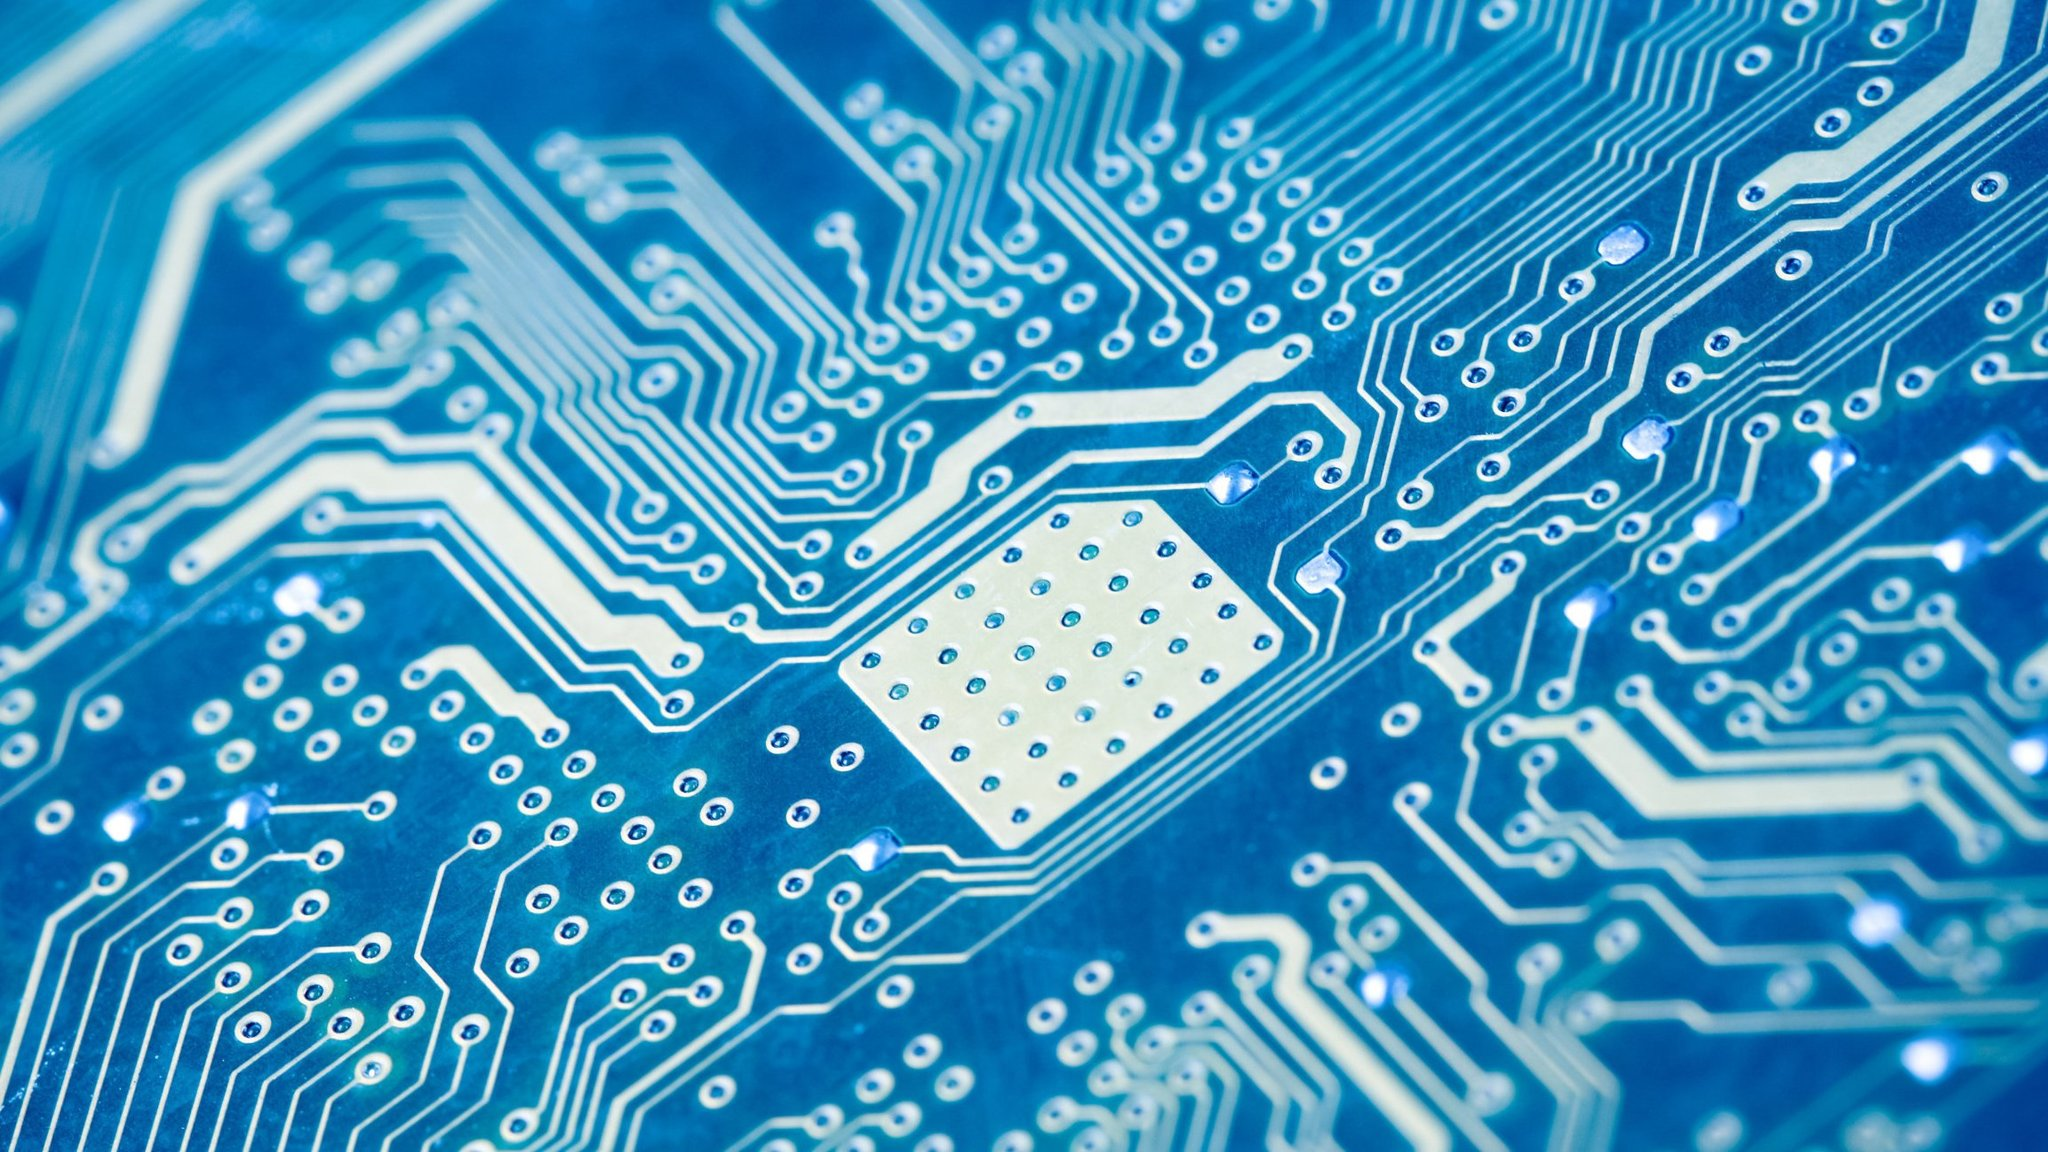
\includegraphics[height=\paperheight,width=\paperwidth]{../03_img/processor.jpg}
			};
		}
		\begin{frame}[plain]
			\vspace*{0.75cm}
			\maketitle
			\vfill
			\begin{center}
				\footnotesize Find all slides on \href{https://github.com/DaWe1992/Applied_ML_Fundamentals}{\linkstyle{GitHub}}
			\end{center}
		\end{frame}
	}
}

% divider page
\newcommand{\makedivider}[1]{
	{
		\beamertemplatenavigationsymbolsempty
		\usebackgroundtemplate{%
			\tikz[overlay,remember picture] \node[opacity=0.2, at=(current page.center)] {
  				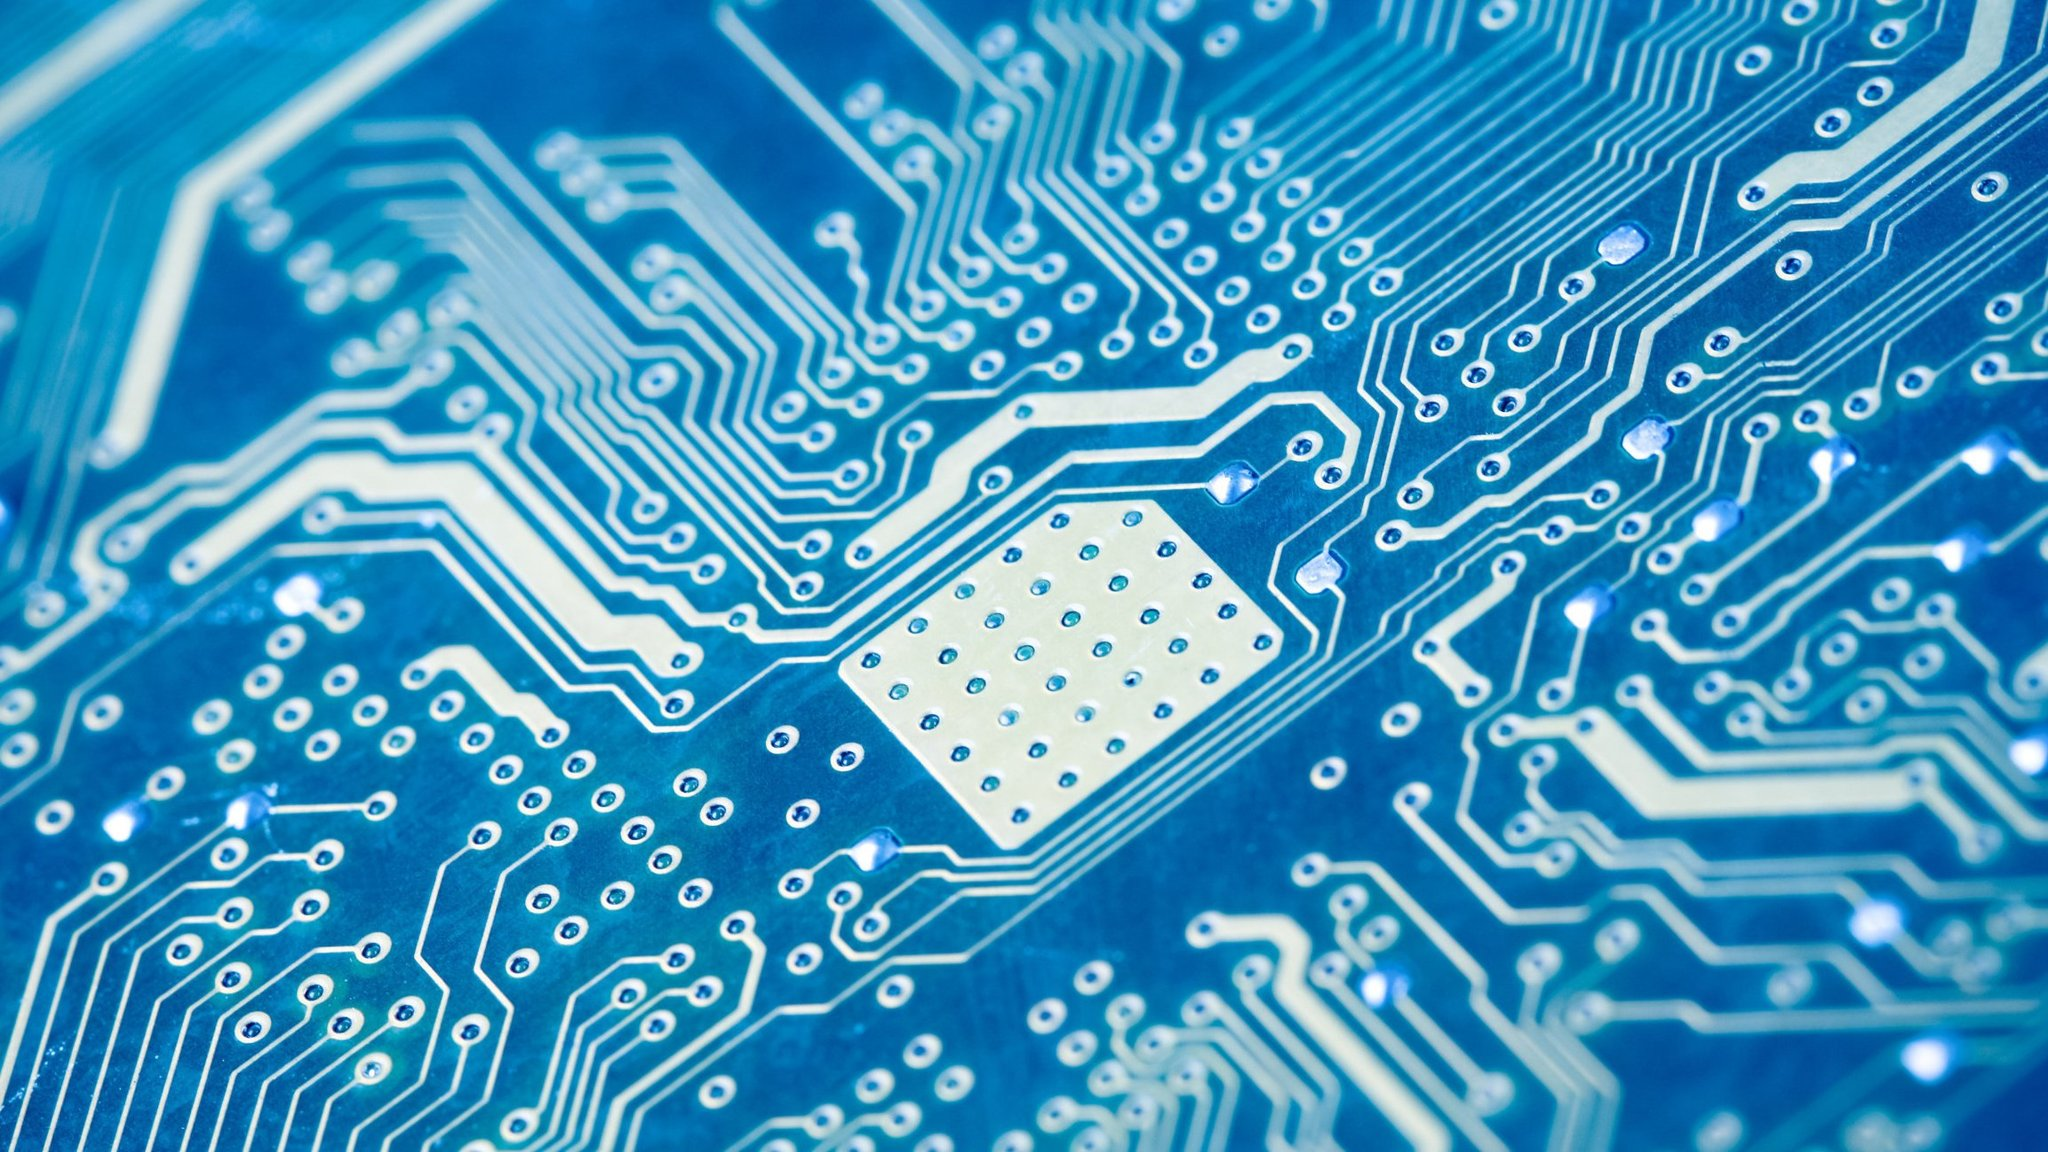
\includegraphics[height=\paperheight,width=\paperwidth]{../03_img/processor.jpg}
			};
		}
		\begin{frame}[plain]
			\vfill
			\begin{boxBlue}
				\centering
				\textbf{Section:} \\
				\large \highlight{#1}
			\end{boxBlue}
			\vfill
			\centering
			
\includegraphics[scale=0.05]{../03_img/logo_dhbw.png}
			\vfill
		\end{frame}
	}
}

% overview page
\newcommand{\makeoverview}[1]{
	\begin{frame}{Lecture Overview}{}
		\begin{tabbing}
			\hspace*{3.5cm}\= \kill
			\ifnum #1=1 \highlight{\textbf{Unit I:}} \else \textbf{Unit I:} \fi
			\> \ifnum #1=1 \highlight{Machine Learning Introduction} \else Machine Learning Introduction \fi \\
		\end{tabbing}
	\end{frame}
}

% thank you page
\newcommand{\makethanks}{
	{\beamertemplatenavigationsymbolsempty
	\begin{frame}[plain]
		\vfill
		\begin{boxBlue}
			\centering
			\Large \highlight{Thank you very much for the attention!}
		\end{boxBlue}
		
		\vfill\footnotesize
		\begin{tabbing}
			\hspace*{1.5cm}\= \kill
			\highlight{Topic:} 	\> \inserttitle \\
			\highlight{Date:} 	\> \insertdate
		\end{tabbing}
		
		\vfill
		\highlight{Contact:} \\
		\insertauthor\ (D062271) \\
		\insertinstitute \\
		\href{mailto:daniel.wehner@sap.com}{\linkstyle{daniel.wehner@sap.com}}
		
		\vfill\normalsize
		\begin{center}
			\large\highlight{Do you have any questions?}
		\end{center}
		\vfill
	\end{frame}}
}

% global pfgplots settings
% --------------------------------------------------------------------------------------------------------
\pgfplotsset{
	% allow filtering of data for pgfplots
	discard if/.style 2 args={
        		x filter/.code={
            		\edef\tempa{\thisrow{#1}}
            		\edef\tempb{#2}
            		\ifx\tempa\tempb
                		\def\pgfmathresult{inf}
            		\fi
        		}
    	},
    	discard if not/.style 2 args={
        		x filter/.code={
            		\edef\tempa{\thisrow{#1}}
            		\edef\tempb{#2}
            		\ifx\tempa\tempb
            		\else
                		\def\pgfmathresult{inf}
            		\fi
        		}
    	}
}


% ====================================================
% ====================================================
% PRESENTATION DATA
% ====================================================
% ====================================================

\title[Regression]{*** Applied Machine Learning Fundamentals *** Regression}
\institute[SAP\,SE]{SAP\,SE / DHBW Mannheim}
\author{Daniel Wehner, M.Sc.}
\date{Winter term 2020/2021}
\prefix{REG}

% ====================================================
% ====================================================
% BEGIN OF DOCUMENT
% ====================================================
% ====================================================

\begin{document}

% Title frame
%______________________________________________________________________
\maketitlepage


% Lecture Overview
%______________________________________________________________________
\begin{frame}{Lecture Overview}{}
	\makeoverview{5}
\end{frame}


% Agenda
%______________________________________________________________________
\begin{frame}{Agenda for this Unit}
	\begin{multicols}{2}
		\tableofcontents
	\end{multicols}
\end{frame}


% Section: Introduction
%______________________________________________________________________
\section{Introduction}
\makedivider{Introduction}

% Subsection: What is Regression?
% --------------------------------------------------------------------------------------------------------
\subsection{What is Regression?}

% Regression
\begin{frame}{Regression}{}
	\vspace*{-6mm}
	\begin{tabbing}
		\hspace*{7cm}\= \kill
		\highlight{Type of target variable}		\> Continuous 		\\[1mm]
		\highlight{Type of training information} 	\> Supervised 		\\[1mm]
		\highlight{Example Availability}			\> Batch learning	\\[1mm]
	\end{tabbing}
	
	\vspace*{-7mm}
	\footnotesize
	\begin{boxBlueNoFrame}
		\textbf{Algorithm sketch:} Given the training data $\mathcal{D}$, the algorithm derives
		a function of the type
	
		\vspace*{-6mm}
		\begin{equation}
			h_{\bm{\theta}}(\bm{x}) = \theta_0 + \theta_1 x_1 + \dots + \theta_{m} x_{m}
				\qquad \bm{x} \in \mathbb{R}^{m}, \bm{\theta} \in \mathbb{R}^{m+1}
		\end{equation}

		from the data. $\bm{\theta}$ is the parameter vector containing the coefficients to be estimated by the regression
 		algorithm. Once $\bm{\theta}$ is learned, it can be used for prediction. 
	\end{boxBlueNoFrame}
\end{frame}


% Example Data Set: Revenues
\begin{frame}{Example Data Set: Revenues}{}
	\divideTwo{0.44}{
		\begin{figure}
	\centering
	\begin{tikzpicture}
    
  	  \begin{axis}[
			scale=0.6,
			axis lines=middle,
			xlabel={\textbf{Marketing Expenses} $x_1$},
			ylabel={\textbf{Revenue} $y$},
    			xtick={\empty},ytick={\empty},
			x label style={at={(axis description cs:0.5,-0.3)},anchor=south},
    			y label style={at={(axis description cs:0,1)},anchor=south}
		]

			\pgfplotstableread{05_regression/05_data/data_regression_marketing_expenses.txt} \datatable
			\addplot[only marks,mark=*,mark size=2,draw=myblue1,fill=lightgray] table[x=x,y=y] from \datatable;
		\end{axis}
	\end{tikzpicture}
\end{figure}
	}{0.55}{
		\begin{itemize}
			\item Find a linear function:
			\begin{equation*}
				h_{\bm{\theta}}(\bm{x}) = \theta_0 + \theta_1 x_1 + \dots + \theta_{m} x_{m}
			\end{equation*}
			\item Usually: $x_0 = 1$:
		\end{itemize}
		\begin{align*}
			\bm{\widehat{x}} \in \mathbb{R}^{m+1}
				&= [1\ \bm{x}]^{\intercal} \\
			h_{\bm{\theta}}(\bm{\widehat{x}}) = \sum_{j=0}^{m} \theta_j x_j
				&= \bm{\theta}^{\intercal} \bm{\widehat{x}}
		\end{align*}
	}
\end{frame}


% Subsection: Least Squares Error Function
% --------------------------------------------------------------------------------------------------------
\subsection{Least Squares Error Function}

% Error Function for Regression
\begin{frame}{Error Function for Regression}{}
	\begin{itemize}
		\item We need an error function $\mathcal{J}(\bm{\theta})$ in order to know how good the function fits:
		\begin{equation}
			\mathcal{J}(\bm{\theta}) = \frac{1}{2n} \sum_{i=1}^n (h_{\bm{\theta}}(\bm{\widehat{x}}^{(i)}) - y^{(i)})^2
		\end{equation}
		\item We want to minimize $\mathcal{J}(\bm{\theta})$:
		\begin{equation*}
			\min_{\bm{\theta}} \frac{1}{2n} \sum_{i=1}^n (h_{\bm{\theta}}(\bm{\widehat{x}}^{(i)}) - y^{(i)})^2
		\end{equation*}
		\item This is \highlight{ordinary least squares (OLS)}
	\end{itemize}
\end{frame}


% Error Function Intuition
\begin{frame}{Error Function Intuition}{}
	\bubble{12}{9}{
		\scriptsize Why the \textbf{square} \\[-2mm]
		\scriptsize in the error function?
	}
	\vspace*{2mm}
	\begin{figure}
	\centering
	\begin{tikzpicture}[
		scale=0.8
	]
		
		% error bars
		\draw[dashed] (1,3) -- (1,1.3);
		\draw[dashed] (3,1) -- (3,1.9);
		\draw[dashed] (6,2) -- (6,2.8);
		\draw[dashed] (8,3) -- (8,3.4);
		\draw[dashed] (9,4.5) -- (9,3.7);

		% curly brace
		\draw [decorate,decoration={brace,amplitude=3pt,mirror,raise=2pt},yshift=0pt]
			(1,1.4) -- (1,2.8) node [black,midway,xshift=0.8cm] {};

		% data points
		\foreach \x/\y in {1/3,3/1,6/2,8/3,9/4.5}{
			\draw[myblue1,fill=lightgray] (\x,\y) circle (5pt);
		}

		% regression function
		\draw[very thick,myblue1] (0,1) -- (10,4)
			node[right,myblue1] {$h_{\bm{\theta}}(\bm{\widehat{x}}) = \bm{\theta}^{\intercal}\bm{\widehat{x}}$};

		% coordinate system
		\draw[thick,-stealth] (0,0) -- (10,0) node[right] {$x$};
		\draw[thick,-stealth] (0,0) -- (0,5) node[above] {$y$};

		% ticks and ticks labels
		\foreach \x in {1,2,3,...,9}{
			\draw (\x,0) -- (\x,-0.15);
			\node at (\x,-0.5) {\tiny \x};
		}

		\foreach \y in {1,2,...,4}{
			\draw (0.0,\y) -- (-0.15,\y);
			\node at (-0.5,\y) {\tiny \y};
		}

		\node at (1.25,3.75) {$y^{(i)}$};
		\node at (5,5.25) {$(h_{\bm{\theta}}(\widehat{x}^{(i)}) - y^{(i)})$};
		\draw[stealth-stealth] (5,4.75) .. controls (4,3) .. (1.3,2.15);
		\node at (1,-1.25) {$x^{(i)}$};

	\end{tikzpicture}
\end{figure}
\end{frame}


% Section: Solutions to Regression
%______________________________________________________________________
\section{Solutions to Regression}
\makedivider{Solutions to Regression}

% Subsection: Closed-Form Solutions and Normal Equation
% --------------------------------------------------------------------------------------------------------
\subsection{Closed-Form Solutions and Normal Equation}

% Closed-Form Solutions
\begin{frame}{Closed-Form Solutions}{}
	\bubble{0.5}{5.5}{
		\scriptsize sample mean $\overline x$
	}
	\begin{itemize}
		\item Usual approach (for two unknowns): Calculate $\theta_0$ and $\theta_1$ according to
		\begin{equation}
			\theta_0 = \overline{y} - \theta_1 \overline{x} \qquad\qquad
			\theta_1 = \frac{\sum_{i=1}^n (x^{(i)} - \overline{x}) \cdot
				(y^{(i)} - \overline{y})}{\sum_{i=1}^n (x^{(i)} - \overline{x})^2}
		\end{equation}
		\item \highlight{`Normal equation'} (scales to arbitrary dimensions):
		\begin{equation}
			\bm{\theta} = \underbracket{
				(\bm{\widehat{X}}^{\intercal} \bm{\widehat{X}})^{-1} \bm{\widehat{X}}^{\intercal}
			}_{\substack{\text{Moore-Penrose} \\ \text{pseudo-inverse}}} \bm{y}
		\end{equation}
		$\bm{\widehat{X}}$ is called `design matrix' or `regressor matrix'
	\end{itemize}
\end{frame}


% Design Matrix / Regressor Matrix
\begin{frame}{Design Matrix / Regressor Matrix}{}
	\bubble{12}{4.5}{
		\scriptsize In the following \\
		\scriptsize $\bm{\widehat{X}} \equiv \bm{X}$
	}
	\begin{itemize}
		\item The design matrix $\bm{\widehat{X}} \in \mathbb{R}^{n \times (m + 1)}$ looks as follows:
		\footnotesize
		\begin{equation}
			\bm{\widehat{X}} =
			\begin{pmatrix}
  				1 & x_1^{(1)} & x_2^{(1)} & \cdots & x_m^{(1)} \\
				1 & x_1^{(2)} & x_2^{(2)} & \cdots & x_m^{(2)} \\
				1 & x_1^{(3)} & x_2^{(3)} & \cdots & x_m^{(3)} \\
				\vdots & \vdots & \vdots & \ddots & \vdots \\
				1 & x_1^{(n)} & x_2^{(n)} & \cdots & x_m^{(n)} \\
 			\end{pmatrix}
		\end{equation}
		\normalsize
		\item And the $n \times 1$ label vector:
		\footnotesize
		\begin{equation*}
			 \bm{y} =
			 \begin{pmatrix}
				y^{(1)}, y^{(2)}, y^{(3)}, \dots, y^{(n)}
			\end{pmatrix}^{\intercal}
		\end{equation*}
	\end{itemize}
\end{frame}


% Derivation of the Normal Equation
\begin{frame}{Derivation of the Normal Equation}{}\optional
	\begin{itemize}
		\item The derivation involves a bit of linear algebra
		\item Step \ding{182}: Rewrite $\mathcal{J}(\bm{\theta})$ in matrix-vector notation:
		\begin{align*}
			\mathcal{J}(\bm{\theta})
				&= \nicefrac{1}{2}(\bm{X} \bm{\theta} - \bm{y})^{\intercal} (\bm{X} \bm{\theta} - \bm{y}) \\
				&= \nicefrac{1}{2}((\bm{X} \bm{\theta})^{\intercal} - \bm{y}^{\intercal}) (\bm{X} \bm{\theta} - \bm{y}) \\
				&= \nicefrac{1}{2}((\bm{X} \bm{\theta})^{\intercal} \bm{X} \bm{\theta} - (\bm{X} \bm{\theta})^{\intercal} \bm{y}
					- \bm{y}^{\intercal} (\bm{X} \bm{\theta}) + \bm{y}^{\intercal} \bm{y}) \\
				&= \nicefrac{1}{2}(\bm{\theta}^{\intercal} \bm{X}^{\intercal} \bm{X} \bm{\theta}
					- 2 (\bm{X} \bm{\theta})^{\intercal} \bm{y} + \bm{y}^{\intercal} \bm{y})
		\end{align*}
		\item To be continued...
	\end{itemize}
\end{frame}


% Derivation of the Normal Equation (Ctd.)
\begin{frame}{Derivation of the Normal Equation (Ctd.)}{}\optional
	\begin{itemize}
		\item Step \ding{183}: Calculate the derivative of $\mathcal{J}(\bm{\theta})$ and set it to zero:
		\begin{align*}
			\nabla_{\bm{\theta}}\mathcal{J}(\bm{\theta})
				&= \nicefrac{1}{2}(2 \bm{X}^{\intercal} \bm{X} \bm{\theta} - 2 \bm{X}^{\intercal} \bm{y}) \overset{!}{=} \bm{0} \\	
				&\Leftrightarrow \bm{X}^{\intercal} \bm{X} \bm{\theta} = \bm{X}^{\intercal} \bm{y}
		\end{align*}
		\item If $\bm{X}^{\intercal} \bm{X}$ is invertible, we can multiply both sides by
			$(\bm{X}^{\intercal} \bm{X})^{-1}$:
		\vspace*{3mm}
		\begin{boxBlueNoFrame}
			\highlight{Normal equation:}
			\begin{equation*}
				\bm{\theta} = (\bm{X}^{\intercal} \bm{X})^{-1} \bm{X}^{\intercal} \bm{y}
			\end{equation*}
		\end{boxBlueNoFrame}
	\end{itemize}
\end{frame}


% Problems with Matrix Inversion?
\begin{frame}{Problems with Matrix Inversion?}{}
	\begin{itemize}
		\item What if $(\bm{X}^{\intercal} \bm{X})^{-1}$ does not exist?
		\item Problems and solutions:
		\begin{enumerate}
			\item Linearly dependent (redundant) features or design matrix does not have full rank? 
				(E.\,g. size in m$^2$ and size in feet$^2$) \\
				\highlight{$\Rightarrow$ Delete correlated features}
			\item Too many features ($m > n$)? \\
				\highlight{$\Rightarrow$ Delete features (e.\,g. using PCA) / add training examples}
			\item Other numerical instabilities? \\
				\highlight{$\Rightarrow$ Add a regularization term} (later)
			\item Computationally too expensive? \\
				\highlight{$\Rightarrow$ Use gradient descent}
		\end{enumerate}
	\end{itemize}
\end{frame}


% Subsection: Gradient Descent
% --------------------------------------------------------------------------------------------------------
\subsection{Gradient Descent}

% Gradient Descent
\begin{frame}{Gradient Descent}{}\important
	\begin{itemize}
		\item We want to minimize a smooth function $\mathcal{J} : \mathbb{R}^{m+1} \rightarrow \mathbb{R}$:
		\begin{equation*}
			\min_{\bm{\theta} \in \mathbb{R}^{m+1}} \mathcal{J}(\bm{\theta})
		\end{equation*}
		\item Update the parameters iteratively:
		\begin{equation}
			\bm{\theta}^{(t+1)} \longleftarrow \bm{\theta}^{(t)} -
				\alpha \nabla_{\bm{\theta}} \mathcal{J}(\bm{\theta}^{(t)})
		\end{equation}
		\item where $\alpha > 0$ (\highlight{learning rate}) and $\nabla_{\bm{\theta}} \mathcal{J}(\bm{\theta})$
			is the gradient of $\mathcal{J}(\bm{\theta})$ w.\,r.\,t. $\bm{\theta}$:
		\begin{equation*}
			\nabla_{\bm{\theta}} \mathcal{J}(\bm{\theta}) = 
			\begin{pmatrix}
				\frac{\partial \mathcal{J}(\bm{\theta})}{\partial \theta_0},
				\frac{\partial \mathcal{J}(\bm{\theta})}{\partial \theta_1}, 
				\dots,
				\frac{\partial \mathcal{J}(\bm{\theta})}{\partial \theta_{m}}
			\end{pmatrix}^{\intercal}
		\end{equation*}
	\end{itemize}
\end{frame}


% Data Input Space vs. Hypothesis Space
\begin{frame}{Data Input Space vs. Hypothesis Space}{}
	\divideTwoTop{0.49}{
		\highlight{Data input space}
		\begin{figure}
	\centering
	\begin{tikzpicture}[
		scale=0.6,
		point/.style={
			mark=*,draw=myblue1,fill=lightgray,mark size=3
		}
	]
		\begin{axis}[
			xlabel=$x$,
			ylabel=$y$,
		]
	
			\addplot[no marks,myblue1,very thick]{x};
			\addplot[point] coordinates {(-2,-3)}; 	\addplot[point] coordinates {(0,1.5)};
			\addplot[point] coordinates {(1,2)}; 	\addplot[point] coordinates {(4,3.7)};
			\addplot[point] coordinates {(2,2.5)}; 	\addplot[point] coordinates {(3,1.75)};
			\addplot[point] coordinates {(-4,-3.5)}; 	\addplot[point] coordinates {(-3,-2.25)};
			\addplot[point] coordinates {(-1,-1.2)}; 	\addplot[point] coordinates {(-1.5,-1)};

			\node at (axis cs:2,-2) {$y = \theta_0 + \theta_1 x$};
		\end{axis}

	\end{tikzpicture}
\end{figure}
	}{0.49}{
		\highlight{Hypothesis space $\mathcal{H}$}
		\begin{figure}
	\centering
	\begin{tikzpicture}[
		scale=0.65
	]
		\begin{axis}[
			xlabel=$\theta_0$,
			ylabel=$\theta_1$,
			zlabel=$\mathcal{J}(\bm{\theta})$
		]
	
			\addplot3[
				surf,
				samples=41
			] {x^2+y^2};
		\end{axis}

	\end{tikzpicture}
\end{figure}
	}
\end{frame}


% Data Input Space vs. Hypothesis Space (Ctd.)
\begin{frame}{Data Input Space vs. Hypothesis Space (Ctd.)}{}
	\begin{itemize}
		\item \textbf{Data input space}
		\begin{itemize}
			\item Determined by the $m + 1$ \textbf{attributes} of the data set $x_0, x_1, x_2, \dots, x_m$
			\item Often high-dimensional
		\end{itemize}
		\item \textbf{Hypothesis space $\mathcal{H}$}
		\begin{itemize}
			\item Determined by the \textbf{number of parameters} of the model
			\item Each point in the hypothesis space corresponds to a \textbf{specific assignment of model parameters}
			\item The error function gives information about how good this assignment is
			\item \highlight{Gradient descent is applied in the hypothesis space $\mathcal{H}$}
		\end{itemize}
	\end{itemize}
\end{frame}


% Data Input Space vs. Hypothesis Space (Ctd.)
\begin{frame}{Data Input Space vs. Hypothesis Space (Ctd.)}{}\important
	\begin{figure}
		\centering
		\animategraphics[autoplay,loop,height=5.5cm]{2.5}
			{05_regression/02_img/grad_desc_animation/}{0}{14}
	\end{figure}
\end{frame}


% Visualization of Gradient Descent in 3 Dimensions
\begin{frame}{Visualization of Gradient Descent in 3 Dimensions}{}
	\begin{figure}
	\centering
	\begin{tikzpicture}[
		scale=0.80,
		arr/.style={
			shorten >=0.15mm,shorten <=0.15mm,->,red,very thick
		}
	]
		\begin{axis}[
			xlabel=$\theta_0$,
			ylabel=$\theta_1$,
			zlabel=$\mathcal{J}(\bm{\theta})$
		]
	
			\addplot3[
				surf,
				samples=41
			] {x^2+y^2};

			\draw[draw=red,fill=red] (axis cs:-2,2,40) circle (3pt);
			\draw[arr] (axis cs:-2,2,40) -- (axis cs:-1,2,35);
			\draw[arr] (axis cs:-1,2,35) -- (axis cs:-1,1,30);
			\draw[arr] (axis cs:-1,1,30) -- (axis cs:0,1,25);
			\draw[arr] (axis cs:0,1,25) -- (axis cs:0,0,20);
			\draw[arr] (axis cs:0,0,20) -- (axis cs:0.5,0,15);
		\end{axis}
	\end{tikzpicture}
\end{figure}
\end{frame}


% Versions of Gradient Descent
\begin{frame}{Versions of Gradient Descent}{}
	\begin{itemize}
		\item Assume some training data $\mathcal{D}$: $\{ \bm{x}^{(i)}, y^{(i)} \}_{i=1}^{n}$
		\item Squared error for a \textbf{single} example: $\ell(y_{pred}, y_{true}) = (y_{pred} - y_{true})^2$
		\item Our objective is to minimize the \textbf{total} error:
		\begin{equation*}
			\min_{\bm{\theta} \in \mathbb{R}^{m+1}} \mathcal{J}(\bm{\theta}) =
				\min_{\bm{\theta} \in \mathbb{R}^{m+1}} \sum_{i=1}^n \ell(h_{\bm{\theta}}(\bm{x}^{(i)}), y^{(i)})
		\end{equation*}
		\item Three versions of gradient descent:
		\begin{enumerate}
			\item Batch gradient descent
			\item Stochastic gradient descent
			\item Mini-batch gradient descent
		\end{enumerate}
	\end{itemize}
\end{frame}


% Versions of Gradient Descent (Ctd.)
\begin{frame}{Versions of Gradient Descent (Ctd.)}{}
	\begin{itemize}
		\item \highlight{Batch gradient descent}: Compute gradient based on \textbf{\underline{ALL}} data points
		\begin{equation}
			\bm{\theta}^{(t+1)} \longleftarrow \bm{\theta}^{(t)} - \alpha
				\textcolor{myblue1}{\bm{\sum_{i=1}^{n}}} \nabla \ell(h_{\bm{\theta}^{(t)}}(\bm{x}^{(i)}), y^{(i)})
		\end{equation}
		
		\item \highlight{Stochastic gradient descent}: Compute gradient based on a \textbf{\underline{SINGLE}} data point
			\Highlight{(pick training example randomly and not sequentially!)}
		\item \texttt{For} $i \in \{1, \dots, n\}$ \texttt{do:}
		\vspace*{-3mm}
		\begin{equation}
			\bm{\theta}^{(t+1)} \longleftarrow \bm{\theta}^{(t)} - \alpha \nabla \ell(h_{\bm{\theta}^{(t)}}(\bm{x}^{(i)}), y^{(i)})
		\end{equation}
	\end{itemize}
\end{frame}


% Solving linear Regression using Gradient Descent
\begin{frame}{Solving linear Regression using Gradient Descent}{}
	\begin{itemize}
		\item Randomly initialize $\bm{\theta}$
		\item To minimize the error, keep changing $\bm{\theta}$ according to:
		\begin{equation}
			\bm{\theta}^{(t+1)} \longleftarrow \bm{\theta}^{(t)}
				- \alpha \nabla_{\bm{\theta}}\mathcal{J}(\bm{\theta}^{(t)})
		\end{equation}
		\item We need to calculate $\nabla_{\theta_j}\mathcal{J}(\bm{\theta}^{(t)})$: 
			{\footnotesize (based on a single example)}
		{\footnotesize
		\begin{align}
			\frac{\partial}{\partial \theta_j} \mathcal{J}(\bm{\theta})
				&= \frac{\partial}{\partial \theta_j} \frac{1}{2}(h_{\bm{\theta}}(\bm{x}) - y)^2
					= 2 \cdot \frac{1}{2} (h_{\bm{\theta}}(\bm{x}) - y) \cdot \frac{\partial}{\partial \theta_j}
						(h_{\bm{\theta}}(\bm{x}) - y) \\
				&= (h_{\bm{\theta}}(\bm{x}) - y) \cdot \frac{\partial}{\partial \theta_j}
					(\theta_0 x_0 + \dots + \theta_{m} x_{m} - y)
					= \boxed{(h_{\bm{\theta}}(\bm{x}) - y) x_j}
		\end{align}}
	\end{itemize}
\end{frame}


% Solving the introductory Example
\begin{frame}{Solving the introductory Example}{}
	\divideTwo{0.49}{
		\vspace*{4mm}
		\begin{figure}
	\centering
	\begin{tikzpicture}
    		\begin{axis}[
			scale=0.8,
			xlabel={\textbf{M} ($x_1$)},
			ylabel={\textbf{R} ($y$)},
			axis x line=center,
  			axis y line=center,
  			domain=0:8
		]

			\pgfplotstableread{05_regression/05_data/data_regression_marketing_expenses.txt} \datatable
			\addplot[only marks,mark=*,mark size=2,draw=myblue1,fill=lightgray] table[x=x,y=y] from \datatable;

			\addplot[myblue1,ultra thick] {2.9827 * x + 7.4217};
			\draw[myblue1,dashed,very thick] (axis cs:0,15.47499) -- (axis cs:2.7,15.47499);
			\draw[myblue1,dashed,very thick] (axis cs:2.7,0) -- (axis cs:2.7,15.47499);
		\end{axis}

	\end{tikzpicture}
\end{figure}
	}{0.49}{
		\begin{itemize}
			\item $\theta_0 \approx 7.4218$
			\item $\theta_1 \approx 2.9827$
			\item $\mathcal{J}(\bm{\theta}) \approx 446.9584$
			\item $h_{\bm{\theta}}(\bm{x}) = 7.4218 + 2.9827 \cdot x_1$
			\item $R = h_{\bm{\theta}}(2.7) = \bm{\underline{\underline{15.4750}}}$
		\end{itemize}
	}
\end{frame}


% Disadvantage of Gradient Descent
\begin{frame}{Disadvantage of Gradient Descent}{}
	\begin{figure}
\centering
\begin{tikzpicture}
    
    \begin{axis}[
		scale=0.8,
		xlabel={$\theta$},
		ylabel={$\mathcal{J}(\theta)$},
		domain=-2.5:2,
		x=2cm,
		y=1cm
	]

		\addplot[myblue1,ultra thick,smooth] {0.25 * (x^4 + 0.4 * x^3 - 3 * x^2 + x + 2)};
		\node[align=center,gray] at (axis cs:-1.25,1) {\textbf{Global}\\ \textbf{Optimum}};
		\node[align=center,gray] at (axis cs:0.75,1.5) {\textbf{Local}\\ \textbf{Optimum}};
	\end{axis}
\end{tikzpicture}
\end{figure}
\end{frame}


% Section: Probabilistic Regression
%______________________________________________________________________
\section{Probabilistic Regression}
\makedivider{Probabilistic Regression}

% Subsection: Underlying Assumptions
% --------------------------------------------------------------------------------------------------------
\subsection{Underlying Assumptions}

% Probabilistic Regression
\begin{frame}{Probabilistic Regression}{}
	\bubble{2}{10.25}{
		\footnotesize $\beta \equiv$ precision \\[-1mm]
		\footnotesize $\beta = \nicefrac{1}{\sigma^2}$
	}
	\begin{itemize}
		\item \textbf{Assumption 1:} The target function values are generated by adding noise to the function estimate:
		\begin{equation}
			y = h_{\bm{\theta}}(\bm{x}) + \varepsilon
		\end{equation}
		\item \textbf{Assumption 2:} The noise is a Gaussian random variable:
		\begin{align}
			\varepsilon &\thicksim \mathcal{N}(0, \beta^{-1}) \\
			p(y \vert \bm{x}, \bm{\theta}, \beta) &= \mathcal{N}(y \vert h_{\bm{\theta}}(\bm{x}), \beta^{-1})
		\end{align}
		\item \highlight{$y$ is now a random variable!}
	\end{itemize}
\end{frame}


% Probabilistic Regression (Ctd.)
\begin{frame}{Probabilistic Regression (Ctd.)}{}
	\bubble{0.75}{5}{
		\scriptsize \phantom{t|}$\bm{w} \equiv \bm{\theta}$  \\[-1mm]
		\scriptsize \phantom{t||}$t \equiv y$  \\[-1mm]
		\scriptsize $y(x_0, \bm{w}) \equiv h_{\bm{\theta}}(x_0)$
	}
	\vspace*{-2mm}
	\begin{figure}
		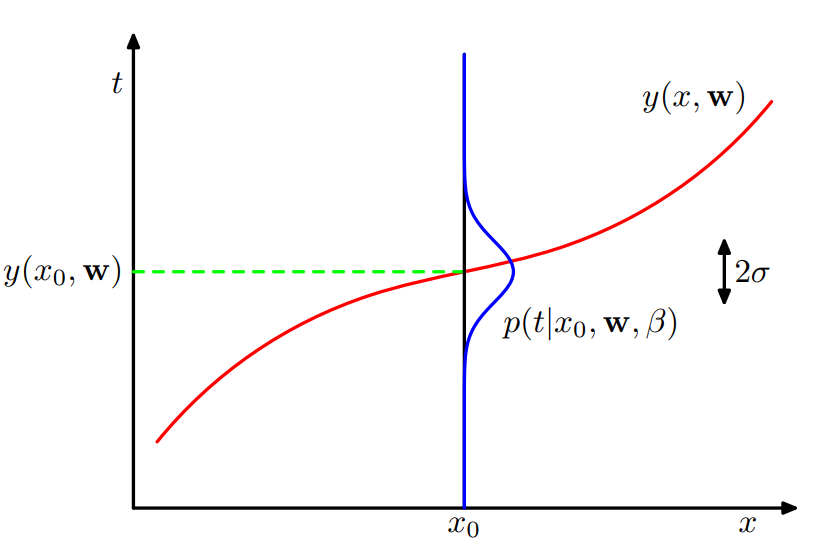
\includegraphics[scale=0.35]{05_regression/02_img/probabilistic_regression}
	\end{figure}
	\begin{center}
		\citeAuthor{cf.}{Bishop.2006}{p. 29; probabilistic regression}
	\end{center}
\end{frame}


% Subsection: Gradient Descent
% --------------------------------------------------------------------------------------------------------
\subsection{Maximum Likelihood Solution}

% Maximum Likelihood Regression
\begin{frame}{Maximum Likelihood Regression}{}
	\begin{itemize}
		\item \textbf{Given:} A labeled set of training data points $\{ (\bm{x}^{(i)}, y^{(i)}) \}_{i=1}^n$
		\item \textbf{Conditional likelihood} (assuming the data is i.\,i.\,d.):
		\begin{align}
			p(\bm{y} \vert \bm{X}, \bm{\theta}, \beta)
				&= \prod_{i=1}^n \mathcal{N}(y^{(i)} \vert h_{\bm{\theta}}(\bm{x}^{(i)}), \beta^{-1}) \\
				&= \prod_{i=1}^n \mathcal{N}(y^{(i)} \vert \bm{\theta}^{\intercal}\bm{x}^{(i)}, \beta^{-1})
		\end{align}
		\item Maximize the likelihood w.\,r.\,t. $\bm{\theta}$ and $\beta$
	\end{itemize}
\end{frame}


% Maximum Likelihood Regression (Ctd.)
\begin{frame}{Maximum Likelihood Regression (Ctd.)}{}
	\bubble{1}{10.5}{
		\scriptsize Remember log-rules?
	}
	Simplify using the \textbf{log}-likelihood:
	\begin{align}
		\log p(\bm{y} \vert \bm{X}, \bm{\theta}, \beta)
			&= \sum_{i=1}^n \log\mathcal{N}(y^{(i)} \vert \bm{\theta}^{\intercal}\bm{x}^{(i)}, \beta^{-1}) \\
			&= \sum_{i=1}^n \left[ \log\left( \frac{\sqrt{\beta}}{\sqrt{2\pi}} \right) - 
				\frac{\beta}{2}(y^{(i)} - \bm{\theta}^{\intercal}\bm{x}^{(i)})^2 \right] \\
			&= \frac{n}{2} \log\beta - \frac{n}{2}\log(2\pi) - \frac{\beta}{2}\sum_{i=1}^n(y^{(i)} -
				\bm{\theta}^{\intercal}\bm{x}^{(i)})^2
	\end{align}
\end{frame}


% Maximum Likelihood Regression (Ctd.)
\begin{frame}{Maximum Likelihood Regression (Ctd.)}{}
	\begin{itemize}
		\item Compute the gradient w.\,r.\,t. $\bm{\theta}$:
		\begin{align*}
			\nabla_{\bm{\theta}} \log p(\bm{y} \vert \bm{X}, \bm{\theta}, \beta) &= \bm{0} \\
			-\beta \sum_{i=1}^n (y^{(i)} - \bm{\theta}^{\intercal} \bm{x}^{(i)})\bm{x}^{(i)} &= \bm{0} \\
			\dots \\
			\bm{\theta}_{ml} &= (\bm{X}^{\intercal}\bm{X})^{-1} \bm{X}^{\intercal} \bm{y}
		\end{align*}
		\item \highlight{Same result as in least squares regression}
	\end{itemize}
\end{frame}


% We have derived the squared Error!
\begin{frame}{We have derived the squared Error!}{}\important
	\begin{boxBlueNoFrame}
		Minimizing the squared error gives the maximum likelihood solution for the parameters $\bm{\theta}$ assuming
		Gaussian noise.
	\end{boxBlueNoFrame}
	\begin{itemize}
		\item The maximum likelihood approach gives rise to the squared error
		\item But it is much more powerful than regular least squares
			\highlight{$\Rightarrow$ We can estimate the uncertainty $\beta$}
	\end{itemize}
	\begin{equation}
		\beta_{ml} = \left( \frac{1}{n} \sum_{i=1}^n
			(y^{(i)} - \bm{\theta}_{ml}^{\intercal} \bm{x}^{(i)})^2 \right)^{-1}
	\end{equation}
\end{frame}


% Section: Basis Function Regression
%______________________________________________________________________
\section{Basis Function Regression}
\makedivider{Basis Function Regression}

% Subsection: General Idea
% --------------------------------------------------------------------------------------------------------
\subsection{General Idea}

% What if the Data is non-linear?
\begin{frame}{What if the Data is non-linear?}{}
	\bubble{2.5}{10.5}{
		\scriptsize The best-fitting function is \\[-2mm]
		\scriptsize obviously \textbf{not a straight line}! \\

		\scriptsize \textbf{What would you do?}
	}
	\divideTwo{0.49}{
		\vspace*{-15mm}
		\begin{itemize}
			\item So far we have fitted straight lines
			\item \Highlight{What if the data is not linear...?}
		\end{itemize}
	}{0.49}{
		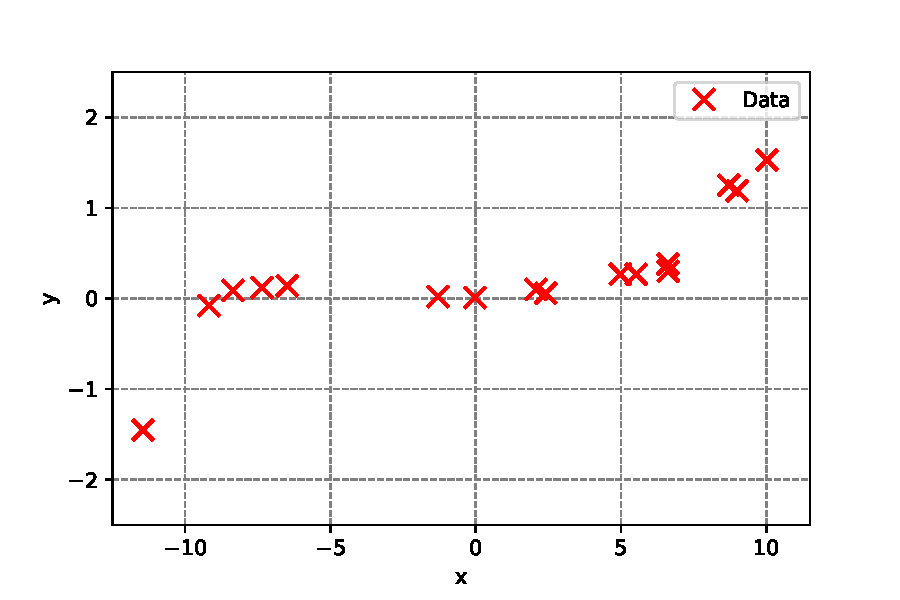
\includegraphics[scale=0.5]{05_regression/02_img/non_linear_data}
	}
\end{frame}


% Basis Functions
\begin{frame}{Basis Functions}{}
	\bubble{2}{7.5}{
		\scriptsize We assume 1-D data
	}
	\begin{itemize}
		\item Remember: \textbf{`When stuck switch to a different perspective'}
		\item We can add \textbf{higher-order} features using \highlight{basis functions $\varphi$}:
		\begin{equation}
			h_{\bm{\theta}}(x) = \sum_{j=0}^p \theta_j\varphi_j(x)
		\end{equation}
		\item There exist several types of basis functions:
		\begin{itemize}
			\item \highlight{linear:} $\varphi_0(x) = 1$ and $\varphi_1(x) = x$
			\item \highlight{polynomial} $\Rightarrow$ see below
			\item \highlight{radial basis functions (RBFs)} $\Rightarrow$ see below
			\item \highlight{Fourier basis}
		\end{itemize}
	\end{itemize}
\end{frame}


% New Design Matrix
\begin{frame}{New Design Matrix}{}
	Applying the basis functions to $\bm{X}$ we get the new design matrix $\bm{\Phi}$:
	
	\footnotesize
	\begin{equation}
		\bm{\Phi} =
		\begin{pmatrix}
			\varphi_0(x^{(1)}) 	& \varphi_1(x^{(1)}) 	& \varphi_2(x^{(1)}) 	& \hdots & \varphi_p(x^{(1)}) 	\\
			\varphi_0(x^{(2)}) 	& \varphi_1(x^{(2)}) 	& \varphi_2(x^{(2)}) 	& \hdots & \varphi_p(x^{(2)}) 	\\
			\vdots 			& \vdots 			& \vdots 			& \ddots & \vdots 			\\
			\varphi_0(x^{(n)}) 	& \varphi_1(x^{(n)}) 	& \varphi_2(x^{(n)}) 	& \hdots & \varphi_p(x^{(n)}) 
		\end{pmatrix}
	\end{equation}
	
	\vspace*{2mm}
	\begin{boxBlueNoFrame}
		\footnotesize
		\highlight{The model is still linear in the parameters, so we can still use the same algorithm as before.}
		\Highlight{This is still linear regression (!!!)}
	\end{boxBlueNoFrame}
\end{frame}


% Subsection: Polynomial Basis Functions
% --------------------------------------------------------------------------------------------------------
\subsection{Polynomial Basis Functions}

% Polynomial Basis Functions
\begin{frame}{Polynomial Basis Functions}{}
	\bubble{8}{6.5}{
		\scriptsize For $N$-D data we would also \\[-2mm]
		\scriptsize include cross-terms!
	}
	\begin{itemize}
		\item A quite frequently used basis function: The \highlight{polynomial basis}
		\begin{align*}
			\varphi_0(x) 			&= 1 	\\
			\varphi_j(x) 			&= x^j	\\
			h_{\bm{\theta}}(x) 	&= \sum_{j=0}^p \theta_j \varphi_j(x) = \theta_0 + \theta_1 x +
									\theta_2 x^2 + \dots + \theta_p x^p
		\end{align*}
		\item Here, $p$ is the degree of the polynomial
		\item Here: $\varphi(x) = [1, x, x^2, x^3, \dots, x^p]$
	\end{itemize}
\end{frame}


% It is still linear!
\begin{frame}{It is still linear!}{}
	\begin{figure}
		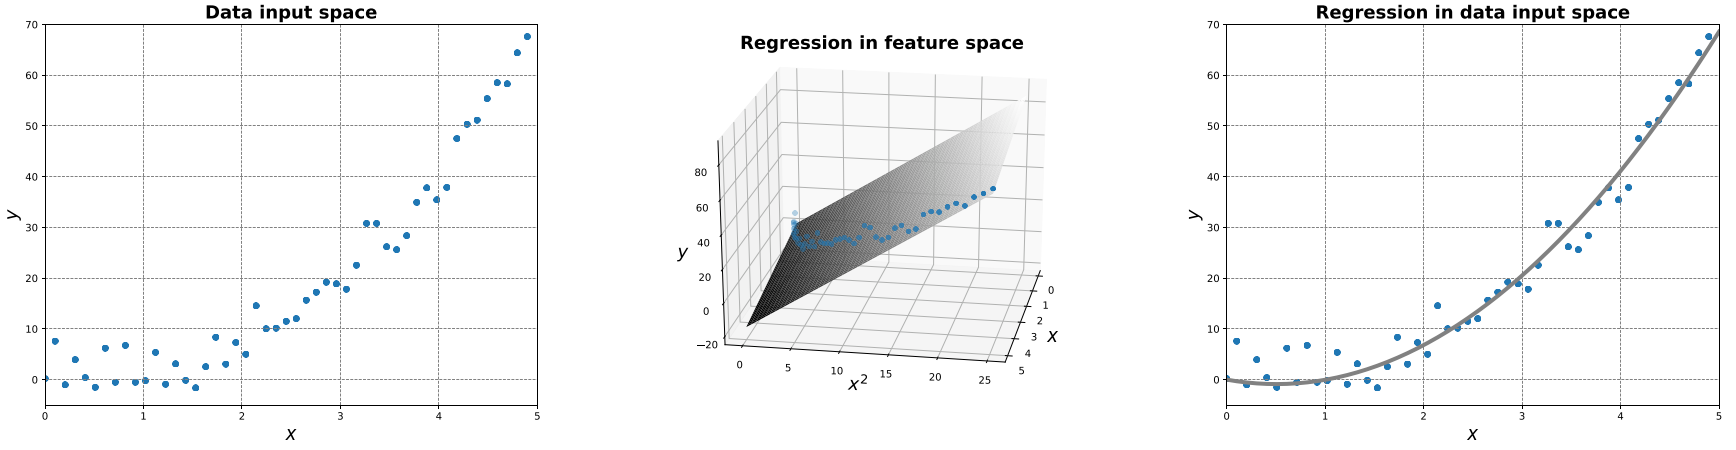
\includegraphics[scale=0.3]{05_regression/02_img/basis_function_regression_visualization}
	\end{figure}
\end{frame}


% It is still linear! (Ctd.)
\begin{frame}{It is still linear! (Ctd.)}{}
	\begin{figure}
		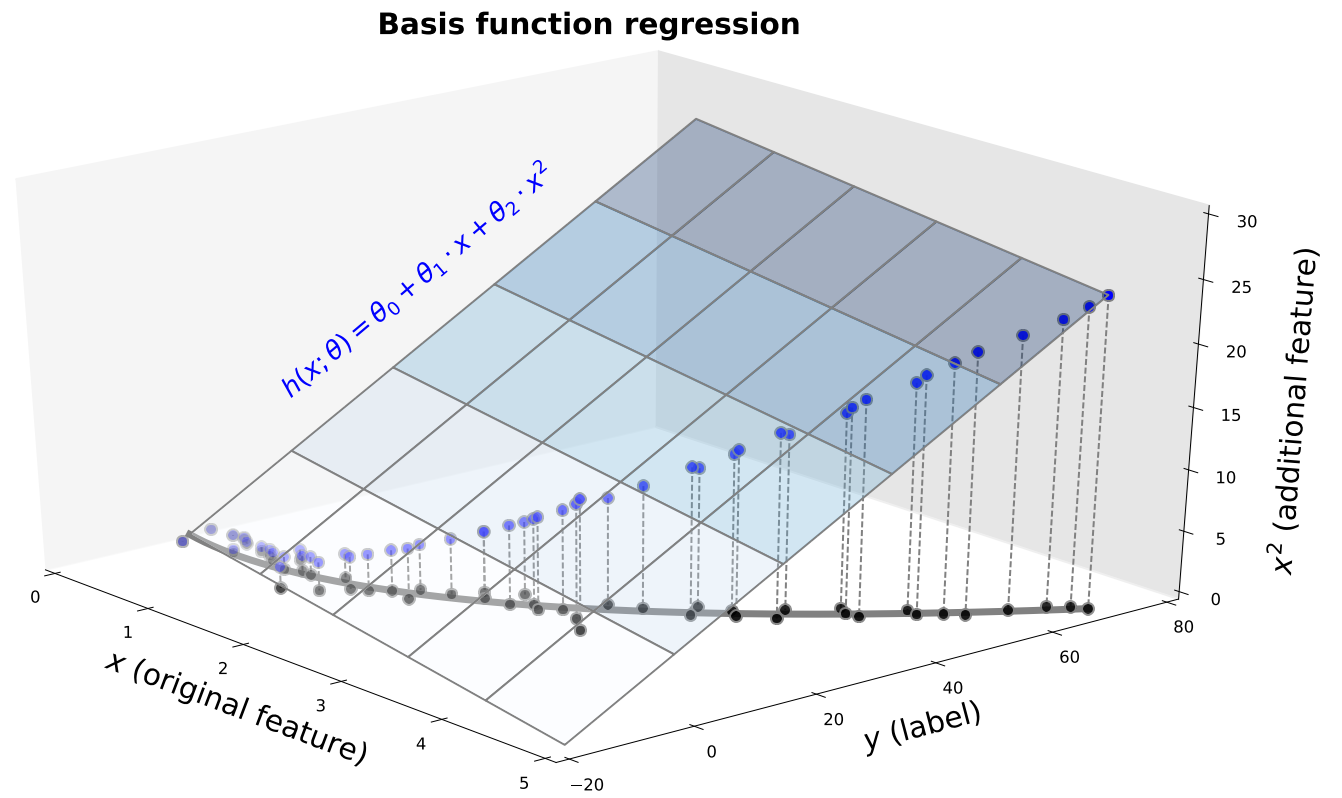
\includegraphics[scale=0.25]{05_regression/02_img/basis_function_regression_visualization_alt}
	\end{figure}
\end{frame}


% Subsection: Radial Basis Functions
% --------------------------------------------------------------------------------------------------------
\subsection{Radial Basis Functions}

% Radial Basis Functions
\begin{frame}{Basis Functions: Radial Basis Functions}{}
	\begin{itemize}
		\item Yet another possible choice of basis function: \highlight{Radial basis functions}
		\begin{align}
			\varphi_0(x) 	&= 1 \\
			\varphi_j(x) 	&= \exp\left\{ - \nicefrac{1}{2} \Vert x - z_j \Vert^2 / 2 \sigma^2 \right\}
		\end{align}
		\item $\{z_j\}$ are the centers of the radial basis functions
		\item $p$ denotes the number of centers / number of radial basis functions
		\item Often we take each data point as a center, so $p = n$
	\end{itemize}
\end{frame}


% Radial Basis Functions (Ctd.)
\begin{frame}{Radial Basis Functions (Ctd.)}{}
	\vspace{-3mm}
	\begin{figure}
		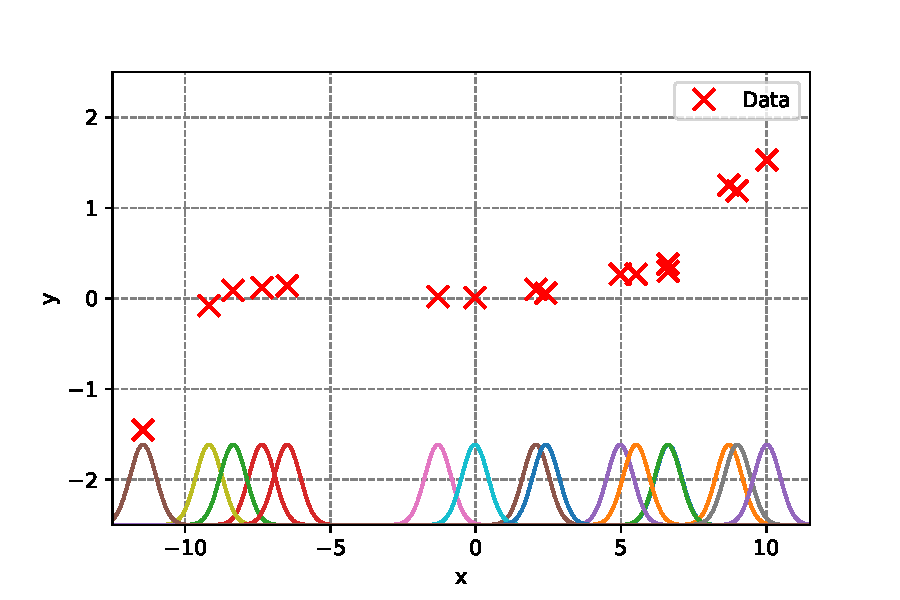
\includegraphics[scale=0.55]{05_regression/02_img/non_linear_data_rbf}
	\end{figure}
\end{frame}


% Subsection: Regularization Techniques
% --------------------------------------------------------------------------------------------------------
\subsection{Regularization Techniques}

% The Danger of too expressive Models...
\begin{frame}{The Danger of too expressive Models...}{}\important
	\divideTwo{0.49}{
		\footnotesize
		Polynomial of degree $p = 16$ \\
		\Highlight{($\skull$ severe overfitting $\skull$)}
		\vspace{-3mm}
		\begin{figure}
			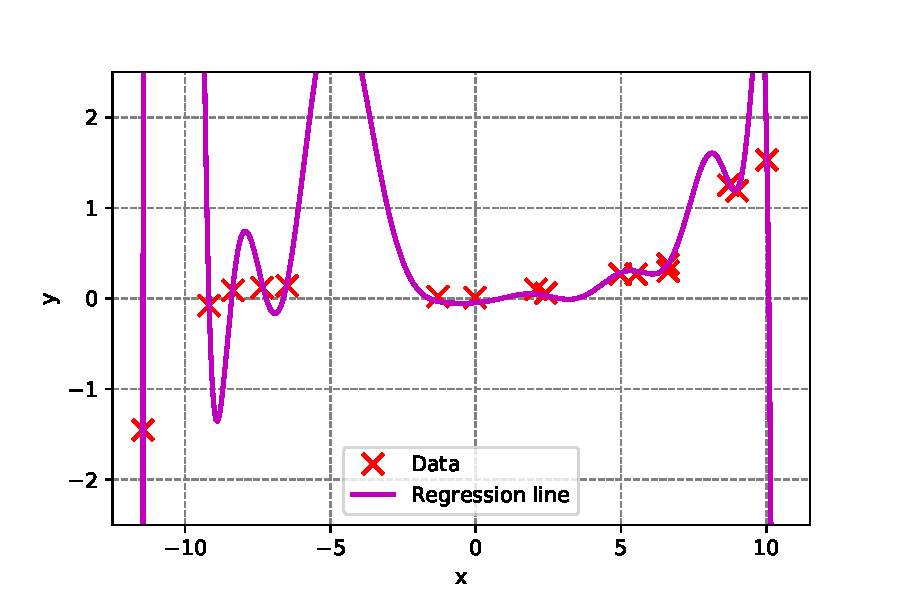
\includegraphics[scale=0.45]{05_regression/02_img/non_linear_data_with_poly_fit}
		\end{figure}
	}{0.49}{
		\footnotesize
		RBF with $\sigma = 1.00, p = n$ \\
		(About right)
		\vspace{-3mm}
		\begin{figure}
			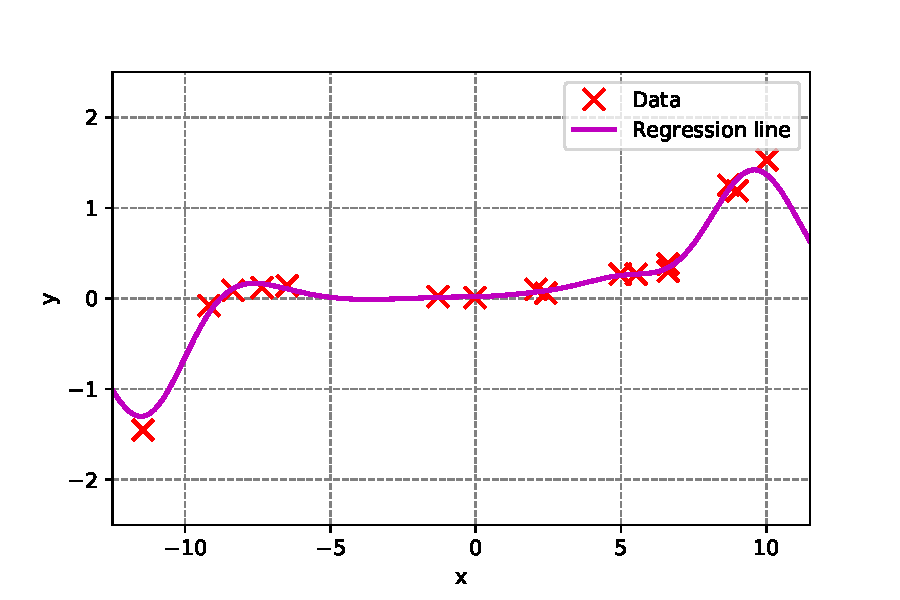
\includegraphics[scale=0.45]{05_regression/02_img/non_linear_data_with_rbf_fit}
		\end{figure}
	}
\end{frame}


% Overfitting vs. Underfitting
\begin{frame}{Overfitting vs. Underfitting}{}
	\begin{itemize}
		\item \textbf{Underfitting}
		\begin{itemize}
			\item The model is not complex enough to fit the data well $\Rightarrow$ \highlight{High bias}
			\item Make the model more complex; adding new examples \Highlight{does not help}
		\end{itemize}
		\item \textbf{Overfitting}
		\begin{itemize}
			\item The model predicts the training data perfectly
			\item But it \Highlight{fails to generalize} to unseen instances $\Rightarrow$ \highlight{High variance}
			\item Decrease the degree of freedom or add more training examples
			\item Also: Try \highlight{regularization}
		\end{itemize}
		\item \highlight{Bias-Variance trade-off}
	\end{itemize}
\end{frame}


% First Solution: Smaller Degree
\begin{frame}{First Solution: Smaller Degree}{}
	\bubble{12}{5}{
		\scriptsize Much better :)
	}
	\vspace*{3mm}
	One solution: Use a \highlight{smaller degree} (here: $p = 3$)
	\vspace{-3mm}
	\begin{figure}
		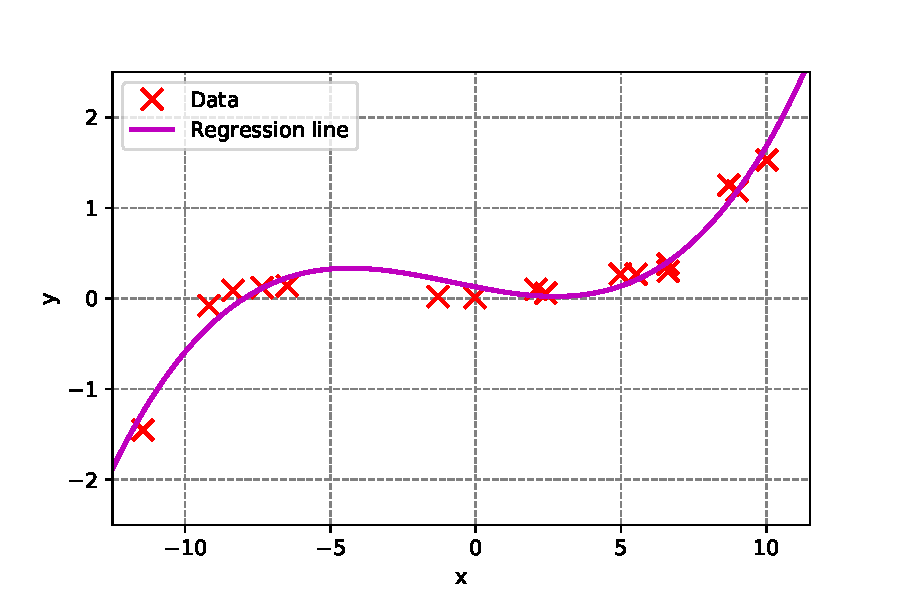
\includegraphics[scale=0.5]{05_regression/02_img/non_linear_data_with_poly_fit_degree_3}
	\end{figure}
\end{frame}


% Second Solution: Regularization
\begin{frame}{Second Solution: Regularization}{}
	\begin{itemize}
		\item Enrich $\mathcal{J}(\bm{\theta})$ with a \highlight{regularization term}
		\item This can \textbf{prevent overfitting} and results in a smoother function \\
			(large values for $\theta_j$ are prevented)
		\item Two forms of regularization, \highlight{L1} and \highlight{L2}:
		\begin{equation*}
			\min_{\bm{\theta}} \mathcal{J}(\bm{\theta}) + \lambda \vert \bm{\theta} \vert
			\quad \rightarrow \text{(\textbf{L1})}
			\qquad\qquad
			\min_{\bm{\theta}} \mathcal{J}(\bm{\theta}) + \lambda \Vert \bm{\theta} \Vert^2
			\quad \rightarrow \text{(\textbf{L2})}
		\end{equation*}
		\vspace*{-3mm}
		\begin{equation*}
			\vert \bm{\theta} \vert = \sum_{j=1}^{m} \vert \theta_j \vert
			\qquad\qquad
			\Vert \bm{\theta} \Vert^2 = \sum_{j=1}^{m} \theta_j^2
		\end{equation*}
		\item $\lambda \ge 0$ controls the \textbf{degree of regularization}
	\end{itemize}
\end{frame}


% Regularization visualized
\begin{frame}{Regularization visualized}{}
	\divideTwo{0.45}{
		\footnotesize
		\begin{itemize}
			\item Here: $\bm{w} \equiv \bm{\theta}$
			\item L1-Regularization \\
				$\Rightarrow$ \highlight{Lasso regression} \\
				\scriptsize (least abs. shrinkage and select. operator) \footnotesize
			\item L2-Regularization \\
				$\Rightarrow$ \highlight{Ridge regression} \\
				\scriptsize (Tikhonov regularization) \footnotesize
			\item The combination of both is called \highlight{elastic net}
		\end{itemize}
	}{0.54}{
		\begin{figure}
			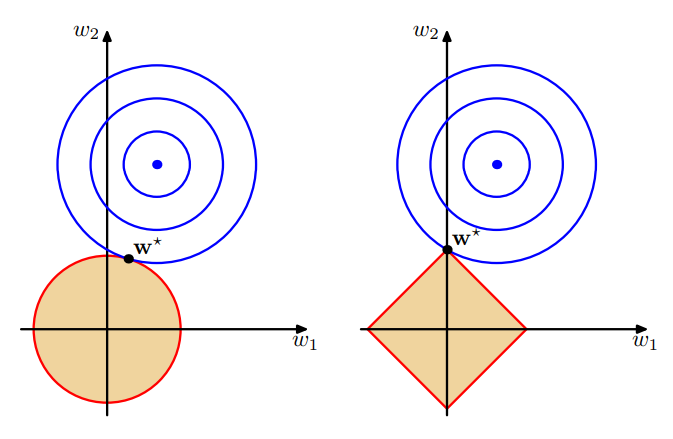
\includegraphics[scale=0.35]{05_regression/02_img/regularization}
		\end{figure}
		\begin{center}
			\citeAuthor{cf.}{Bishop.2006}{p. 146; left: L2, right: L1}
		\end{center}
	}
\end{frame}


% Incorporating Regularization
\begin{frame}{Incorporating Regularization}{}
	\bubble{10}{4.5}{
		\scriptsize The regularization also \\[-2mm]
		\scriptsize helps to overcome numerical issues!
	}
	\vspace*{3mm}
	\begin{itemize}
		\item Normal equation with regularization: \\
		\highlight{(ridge regression)} \\[-0.5mm]
		\begin{equation}
			\bm{\theta} = (\bm{X}^{\intercal} \bm{X}\ \textcolor{myblue1}{+\ \lambda \bm{I}})^{-1}
				\bm{X}^{\intercal} \bm{y}
		\end{equation}
		\item Regularized gradient descent update rule:
		\begin{align*}
			\bm{\theta}^{(t+1)}
				&\longleftarrow \bm{\theta}^{(t)}
					- \alpha \nabla_{\bm{\theta}}\mathcal{J}(\bm{\theta}^{(t)}) \\[2mm]
			\frac{\partial}{\partial \theta_j} \mathcal{J}(\bm{\theta})
				&= (h_{\bm{\theta}}(\bm{x}) - y) x_j\ \textcolor{myblue1}{+\ \lambda \theta_j}
		\end{align*}
	\end{itemize}
\end{frame}


% Polynomial Regression with Regularization
\begin{frame}{Polynomial Regression with Regularization}{}
	\divideTwo{0.49}{
		\textbf{At least better}
		\vspace*{-3mm}
		\begin{figure}
			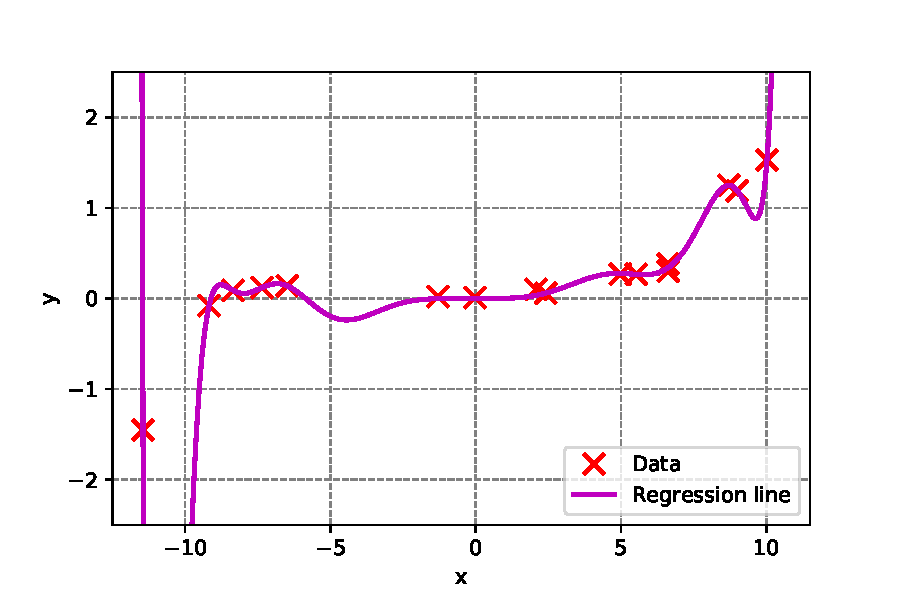
\includegraphics[scale=0.45]{05_regression/02_img/non_linear_data_with_poly_fit_lambda_1000}
		\end{figure}
	}{0.49}{
		\textbf{Way too much regularization}
		\vspace*{-3mm}
		\begin{figure}
			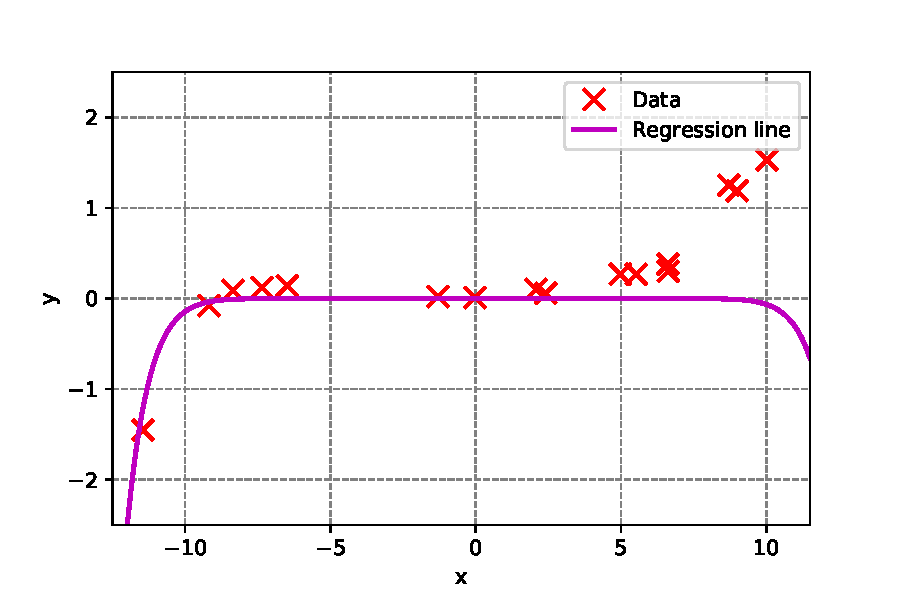
\includegraphics[scale=0.45]{05_regression/02_img/non_linear_data_with_poly_fit_lambda_too_large}
		\end{figure}
	}
\end{frame}


% Section: Wrap-Up
%______________________________________________________________________
\section{Wrap-Up}
\makedivider{Wrap-Up}

% Subsection: Summary
% --------------------------------------------------------------------------------------------------------
\subsection{Summary}

% Summary
\begin{frame}{Summary}{}
	\begin{itemize}
		\item Regression predicts \textbf{continuous target variables}
		\item The algorithm minimizes the \textbf{(mean) squared error}
		\item Minimizing the squared error gives the \textbf{maximum likelihood solution}
		\item \textbf{Two approaches:}
		\begin{enumerate}
			\item Normal equation
			\item (Batch / stochastic / mini-batch) gradient descent
		\end{enumerate}
		\item Probabilistic regression allows to \textbf{quantify the uncertainty of the model}
		\item Use \textbf{basis functions} to fit non-linear regression lines
		\item \textbf{Regularization} is important
	\end{itemize}
\end{frame}


% Subsection: Self-Test Questions
% --------------------------------------------------------------------------------------------------------
\subsection{Self-Test Questions}

% Self-Test Questions
\begin{frame}{Self-Test Questions}{}\important
	\begin{enumerate}
		\item What is the goal of regression?
		\item What can you do if matrix inversion fails for the normal equation?
		\item What is a suitable cost function for regression? Where does it come from?
		\item Does gradient descent give the exact solution?
		\item What is the advantage of probabilistic regression?
		\item What are basis functions? Why use them? State some examples.
		\item What is overfitting / underfitting?
		\item What is regularization? Why should you apply it?
	\end{enumerate}
\end{frame}


% Subsection: Lecture Outlook
% --------------------------------------------------------------------------------------------------------
\subsection{Lecture Outlook}

\begin{frame}{What's next...?}{}
	\makeoverview{6}
\end{frame}


% Subsection: Recommended Literature and further Reading
% --------------------------------------------------------------------------------------------------------
\subsection{Recommended Literature and further Reading}

% Literature
%______________________________________________________________________
\begin{frame}[allowframebreaks]{Recommended Literature and further Reading}{}
	\footnotesize
	\begin{thebibliography}{2}
		\literature{book}{Bishop.2006}{[1] Pattern Recognition and Machine Learning}
			{Christopher Bishop. Springer. 2006.}{$\rightarrow$ \href{
				http://users.isr.ist.utl.pt/~wurmd/Livros/school/Bishop\%20-\%20Pattern\%20Recognition\%20And\%20Machine\%20Learning\%20-\%20Springer\%20\%202006.pdf
			}{\linkstyle{Link}}, cf. chapter 3.1}
			
		\literature{book}{Murphy.2012}{[2] Machine Learning: A Probabilistic Perspective}
			{Kevin Murphy. MIT Press. 2012.}{$\rightarrow$ \href{
				https://doc.lagout.org/science/Artificial\%20Intelligence/Machine\%20learning/Machine\%20Learning_\%20A\%20Probabilistic\%20Perspective\%20\%5BMurphy\%202012-08-24\%5D.pdf
			}{\linkstyle{Link}}, cf. chapters 1.4.5 and 1.4.7}	
			
		\literature{online}{Ng.2019}{[3] Stanford CS229 course notes}
			{Andrew Ng. Stanford University. 2019.}{$\rightarrow$ \href{
				http://cs229.stanford.edu/summer2019/cs229-notes1.pdf
			}{\linkstyle{Link}}}
			
		\literature{online}{Ng.2008}{[4] Stanford CS229 course recording}
			{Andrew Ng. Stanford University. 2008.}{$\rightarrow$ \href{
				https://www.youtube.com/watch?v=5u4G23_OohI
			}{\linkstyle{Link}}}
	\end{thebibliography}
\end{frame}


% Subsection: Meme of the Day
% --------------------------------------------------------------------------------------------------------
\subsection{Meme of the Day}

% Meme of the Day
\begin{frame}{Meme of the Day}{}
	\begin{figure}
		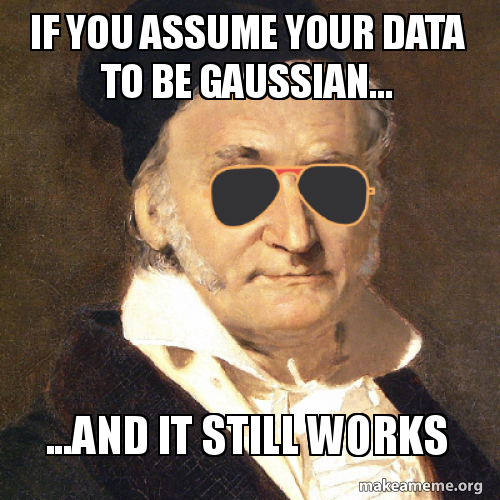
\includegraphics[scale=0.4]{05_regression/02_img/meme_of_the_day}
	\end{figure}
\end{frame}


% Thank you
%______________________________________________________________________
\makethanks

\end{document}